\begin{homeworkProblem}

\textbf{Example I in the Lecture, Section 4}

(a) Implement a Metropolis-Hastings algorithm.

(b) Implement a Hamiltotinn Monte Carlo algorithm

(c) Implement with the Aoceptance-Rejection Method.

(d) Compare the above three algorithms with corresponding pros and cons.

\solution

The target distribution's PDF is
$$f(x)=\dfrac{8}{3\pi\sqrt{5}}\left(1+\dfrac{1}{5}x^2\right)^{-3}, -\infty<x<\infty$$

Since the support of the distribution is $-\infty<x<\infty$, so we first introduce the distribution $Y$ be the deformation of Cauchy distribution. And its PDF and CDF are:
\begin{align*}
g(x) &= \dfrac{1}{\pi\sqrt{5}(1+\frac{1}{5}x^2)} \\
G(x) &= \dfrac{1}{\pi\sqrt{5}}\int_{-\infty}^{x}\dfrac{1}{1+\frac{1}{5}y^2}\dx=\dfrac{1}{\pi}\arctan\left(\dfrac{x}{\sqrt{5}}\right)
\end{align*}
Since $G(x)$ is strictly increasing, by calculating its the inverse function, and sample $U\sim\Unif(0,1)$, we can get the samples $Y$ by:
$$G^{-1}(y) = \sqrt{5}\tan(\pi y), y\in[-0.5,0.5] \Rightarrow XY = \sqrt{5}\tan(\pi (U-0.5))$$

(a) Take the deformation of Cauchy distribution as the proposal distribution, i.e. the one step transition PDF is
$$f_{x,y} = \dfrac{1}{\pi\sqrt{5}(1+\frac{1}{5}y^2)}$$
So the acceptance rate is:
$$a_{x,y}=\min\left(\dfrac{\pi_yf_{y,x}}{\pi_xf_{x,y}},1\right)=\min\left(\left(\dfrac{1+\frac{1}{5}x^2}{1+\frac{1}{5}y^2}\right)^2,1\right)$$
Apply the Metropolis-Hastings algorithm to generate samples as follows:
\begin{figure}[h]
    \centering
    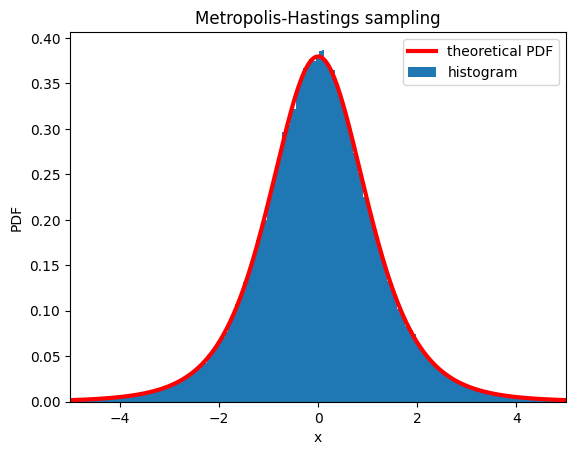
\includegraphics[width=0.5\textwidth]{./figure/p10/MH.png}
\end{figure}

(b) Since $\pi_x$ is a the stationary of the target distribution, and we can ignore the constant form, so the potential energy is
$$U(x)=-\log(\pi_x) = -\log\left(\dfrac{8}{3\pi\sqrt{5}}\right) + 3\log\left(1+\frac{1}{5}x^2\right) \stackrel{\text{ignore const}}{\Rightarrow} U(x)=3\log\left(1+\frac{1}{5}x^2\right)$$
And let the mass be 1, then the Kinetic energy is
$$V(\omega)=\dfrac{1}{2}\omega^2, \quad\text{where } \omega\sim\N(0,1)$$
Thus the Hamiltonian energy is
$$H(x,\omega)=U(x)+V(\omega)=3\log\left(1+\frac{1}{5}x^2\right)+\dfrac{1}{2}\omega^2$$
Initially, set $x_0=0, \omega_0\sim\N(0,1)$, apply the Leapfrog method to sample:
\begin{align*}
\omega_{t+\frac{\delta}{2}} &= \omega_t - \frac{\delta}{2}\cdot \dfrac{\dU(x_t)}{\dx_t} = \omega_t - \frac{\delta}{2}\cdot \dfrac{6x_t}{5+x_t^2} \\
x_{t+\delta} &= x_t + \delta \cdot \dfrac{\dV(\omega_{t+\frac{\delta}{2}})}{\domega_{t+\frac{\delta}{2}}} = x_t + \delta\cdot \omega_{t+\frac{\delta}{2}} \\
\omega_{t+\delta} &= \omega_{t+\frac{\delta}{2}} - \frac{\delta}{2}\cdot \dfrac{\dU(x_{t+\delta})}{\dx_{t+\delta}} = \omega_{t+\frac{\delta}{2}} - \frac{\delta}{2}\cdot \dfrac{6x_{t+\delta}}{5+x_{t+\delta}^2}
\end{align*}
After Leapfrog $L$ steps, we can get the state $(x_L, \omega_L)$. And set $(x_L, -\omega_L)$ to be the proposal distribution. And the accept rate for the Hamiltonian Monte Carlo algorithm is
$$a_{(x_0,\omega_0),(x_L,-\omega_L)}=\min\left(\dfrac{\exp\left(-H(x_L,-\omega_L)\right)}{\exp\left(-H(x_0,\omega_0)\right)}, 1\right)=\min\left(\dfrac{\exp\left(-U(x_L)-V(-\omega_L)\right)}{\exp\left(-U(x_0)-V(\omega_0)\right)}, 1\right)$$
We step the stepsize to be $\delta=0.3, L=15$. One trajectory and sample results are as follows:
\begin{figure}[h]
    \centering
    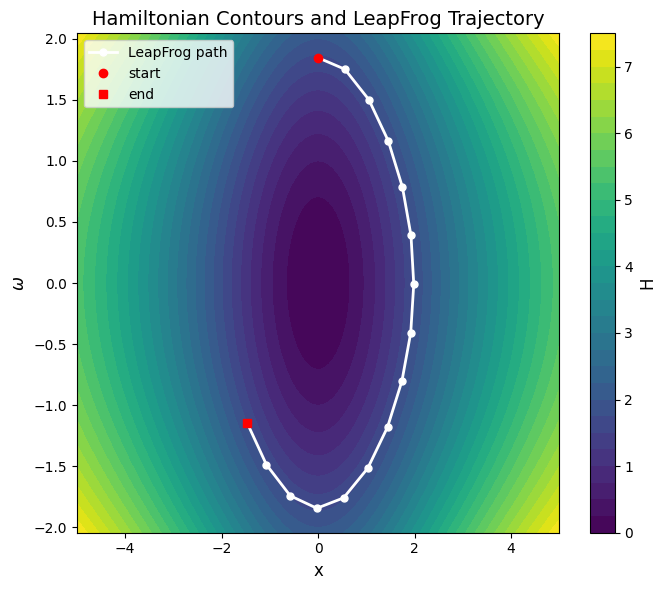
\includegraphics[width=0.49\textwidth]{./figure/p10/trajectory.png}
    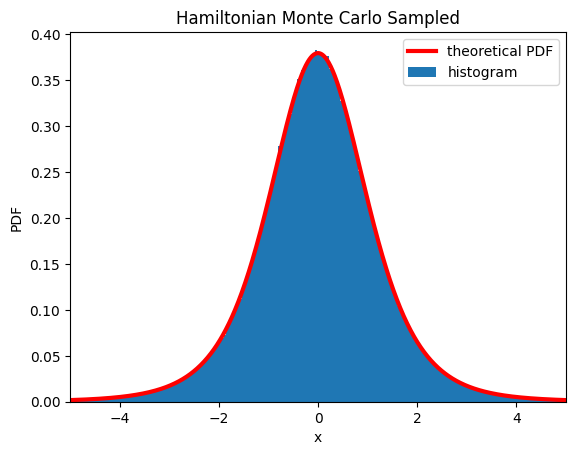
\includegraphics[width=0.49\textwidth]{./figure/p10/Hamiltonian.png}
\end{figure}

(c) As for the acceptance-rejection algorithm, we also use the deformation of Cauchy distribution as the proposal distribution. Let $c$ donate a constant:
$$c = \sup_y\dfrac{f(y)}{g(y)} = \sup_y\dfrac{\frac{8}{3\pi\sqrt{5}}\left(1+\frac{1}{5}y^2\right)^{-3}}{\frac{1}{\pi\sqrt{5}(1+\frac{1}{5}y^2)}}=\dfrac{8}{3}\left.\left(1+\frac{1}{5}y^2\right)^{-2}\right|_{y=0}=\dfrac{8}{3}$$

After sampling the deformation of Cauchy distribution, we can apply the Acceptance-Rejection algorithm to generate the samples: \\
\begin{figure}[htbp]
    \centering
    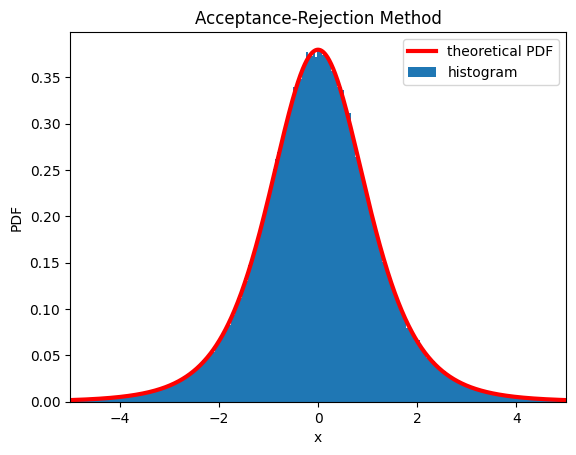
\includegraphics[width=0.5\textwidth]{./figure/p10/accept_reject.png}
\end{figure}

(d) 1. Metropolis-Hastings Algorithm: \\
Advantages: It is highly general-purpose, could applicable to a wide variety of distributions, and it does not require the normalization constant of the target distribution. \\
Disadvantages: Samples are often requires select a suitable distribution, and requires steps to burn up.

2. Hamiltonian Monte Carlo Algorithm: \\
Advantages: Due to the conservation of energy, the acceptance rate should be $1$. But there exists numerical error, however quite close to $1$, which means it has quite high acceptance rate. The samples are efficient, especially in high-dimensional problems. \\
Disadvantages: Requires computation of gradients, increasing implementation complexity. Sensitive to parameters: step size $\delta$ and number of steps for LeapFrog $L$.

3. Acceptance-Rejection Method: \\
Advantages: It produces independent samples, and is simple to implement. If the good envelope function is suitable, it is efficient. \\
Disadvantages: Efficiency depends heavily on the choice of proposal distribution, for example, ours implement has a low acceptance rate, which is only 0.375255.

\end{homeworkProblem}

\newpage